\subsection{加速度計による重力投影と傾斜推定}

車輪オドメトリは車輪が地面を正しく転がることに依存し、ジャイロ積分は角速度バイアスを時間とともに角度誤差へ変える。IMU の中で、ジャイロとは別の情報を与えるのが加速度計である。ただし、加速度計の出力は「物体の並進加速度そのもの」ではない。加速度計が直接測る量は、センサ内部の質量に働く支持力を質量で割った量、すなわち比力（specific force）であり、単位は加速度と同じ $[\mathrm{m/s^2}]$ である。センサが机の上で静止しているとき、慣性座標系での並進加速度は 0 であるにもかかわらず、鉛直上向きにほぼ $9.81\,\mathrm{m/s^2}$ の大きさが出る。この値は、重力によって自由落下しないように机がセンサを支えていることを表す。

慣性座標系を $\{I\}$、IMU に固定した機体系を $\{B\}$ とし、機体系から慣性系への姿勢を $R^I_B$ と書く。慣性系で表した重力加速度を
\begin{equation}
  g^I=\begin{bmatrix}0\\0\\-g\end{bmatrix},
  \qquad
  g=9.80665\,\mathrm{m/s^2}
\end{equation}
とする。IMU 原点の並進加速度を $a^I$ $[\mathrm{m/s^2}]$、加速度計バイアスを $b_a^B$、ノイズを $n_a^B$ とすれば、加速度計の測定値は
\begin{equation}
  a_m^B
  =
  (R^I_B)^\T\left(a^I-g^I\right)+b_a^B+n_a^B
  \label{eq:accelerometer-specific-force}
\end{equation}
で表せる。式\eqref{eq:accelerometer-specific-force}の $a^I-g^I$ が比力である。重力を含む「見かけの加速度」ではなく、重力を差し引いた運動加速度を作るために必要な支持力を、機体系成分で表している。

低速で静止に近い時間帯では、$a^I\simeq0$ とみなせる。このとき
\begin{equation}
  a_m^B\simeq -(R^I_B)^\T g^I
\end{equation}
となり、加速度計は重力ベクトルの向きそのものではなく、重力を打ち消す比力の機体系への投影を返す。したがって、重力の大きさが既知で、並進加速度が小さいという条件が成り立つ間は、加速度計からロール角とピッチ角を幾何的に取り出せる。

ZYX オイラー角で
\begin{equation}
  R^I_B=R_z(\psi)R_y(\theta)R_x(\phi)
\end{equation}
とし、静止に近く、バイアスとノイズをいったん無視する。重力は慣性系の $z$ 軸方向だけを向くので、ヨー角 $\psi$ は重力投影に現れない。計算すると
\begin{align}
  a_m^B
  &\simeq
  - (R^I_B)^\T g^I\\
  &=
  \begin{bmatrix}
    -g\sin\theta\\
    g\sin\phi\cos\theta\\
    g\cos\phi\cos\theta
  \end{bmatrix}.
  \label{eq:accelerometer-gravity-projection}
\end{align}
この式から、ZYX のロール・ピッチ表示で分母 $\sqrt{(a_{m,y}^B)^2+(a_{m,z}^B)^2}$ が 0 に近くない枝では
\begin{align}
  \hat{\phi}_a
  &=
  \operatorname{atan2}\left(a_{m,y}^B,a_{m,z}^B\right),\\
  \hat{\theta}_a
  &=
  \operatorname{atan2}\left(-a_{m,x}^B,
    \sqrt{(a_{m,y}^B)^2+(a_{m,z}^B)^2}\right)
  \label{eq:accelerometer-roll-pitch}
\end{align}
というロール・ピッチ推定値が得られる。式\eqref{eq:accelerometer-roll-pitch}は、重力方向に対して機体がどの向きに傾いているかを、三つの加速度計軸への投影比として定式化したものである。一方、重力ベクトルのまわりの回転であるヨー角は、重力投影だけでは変わらない。加速度計だけでロールとピッチに強い手がかりが得られても、方位までは拘束できない。

平面内のピッチだけに絞ると、導出はさらに見やすい。$\phi=0$、$\psi=0$ とすれば
\begin{equation}
  a_{m,x}^B=-g\sin\theta,\qquad
  a_{m,z}^B=g\cos\theta
\end{equation}
である。したがって
\begin{equation}
  \hat{\theta}_a
  =
  \operatorname{atan2}\left(-a_{m,x}^B,a_{m,z}^B\right)
  =
  \operatorname{atan2}\left(g\sin\theta,g\cos\theta\right)
  =
  \theta
\end{equation}
となる。小角では $a_{m,x}^B\simeq -g\theta$ なので、$x$ 軸の比力を $g$ で割るだけでも傾斜角の一次近似が得られる。この簡潔さが、加速度計を傾斜センサとして使える理由である。

しかし、同じ式は限界も示す。機体が前方へ加速しており、その機体系 $x$ 軸成分を $a_\parallel$ $[\mathrm{m/s^2}]$ とする。重力投影にこの並進成分が加わるので
\begin{equation}
  a_{m,x}^B=a_\parallel-g\sin\theta,\qquad
  a_{m,z}^B=g\cos\theta
\end{equation}
となる。この測定値を静止時の式へそのまま代入すると
\begin{equation}
  \hat{\theta}_a
  =
  \operatorname{atan2}\left(g\sin\theta-a_\parallel,g\cos\theta\right)
  \label{eq:accelerometer-contaminated-tilt}
\end{equation}
である。小角かつ $\abs{a_\parallel}\ll g$ なら
\begin{equation}
  \hat{\theta}_a-\theta
  \simeq
  -\frac{a_\parallel}{g}
\end{equation}
となる。たとえば $a_\parallel=1.6\,\mathrm{m/s^2}$ の加速は、約 $-0.163\,\mathrm{rad}$、すなわち約 $-9.3^\circ$ の偽の傾斜として現れる。ロボットが発進・停止・旋回でこの程度の加速度を受けるなら、加速度計の傾斜値をそのまま姿勢として使うと、真の姿勢変化より大きな誤差を一時的に作る。

\begin{figure}[tb]
\centering
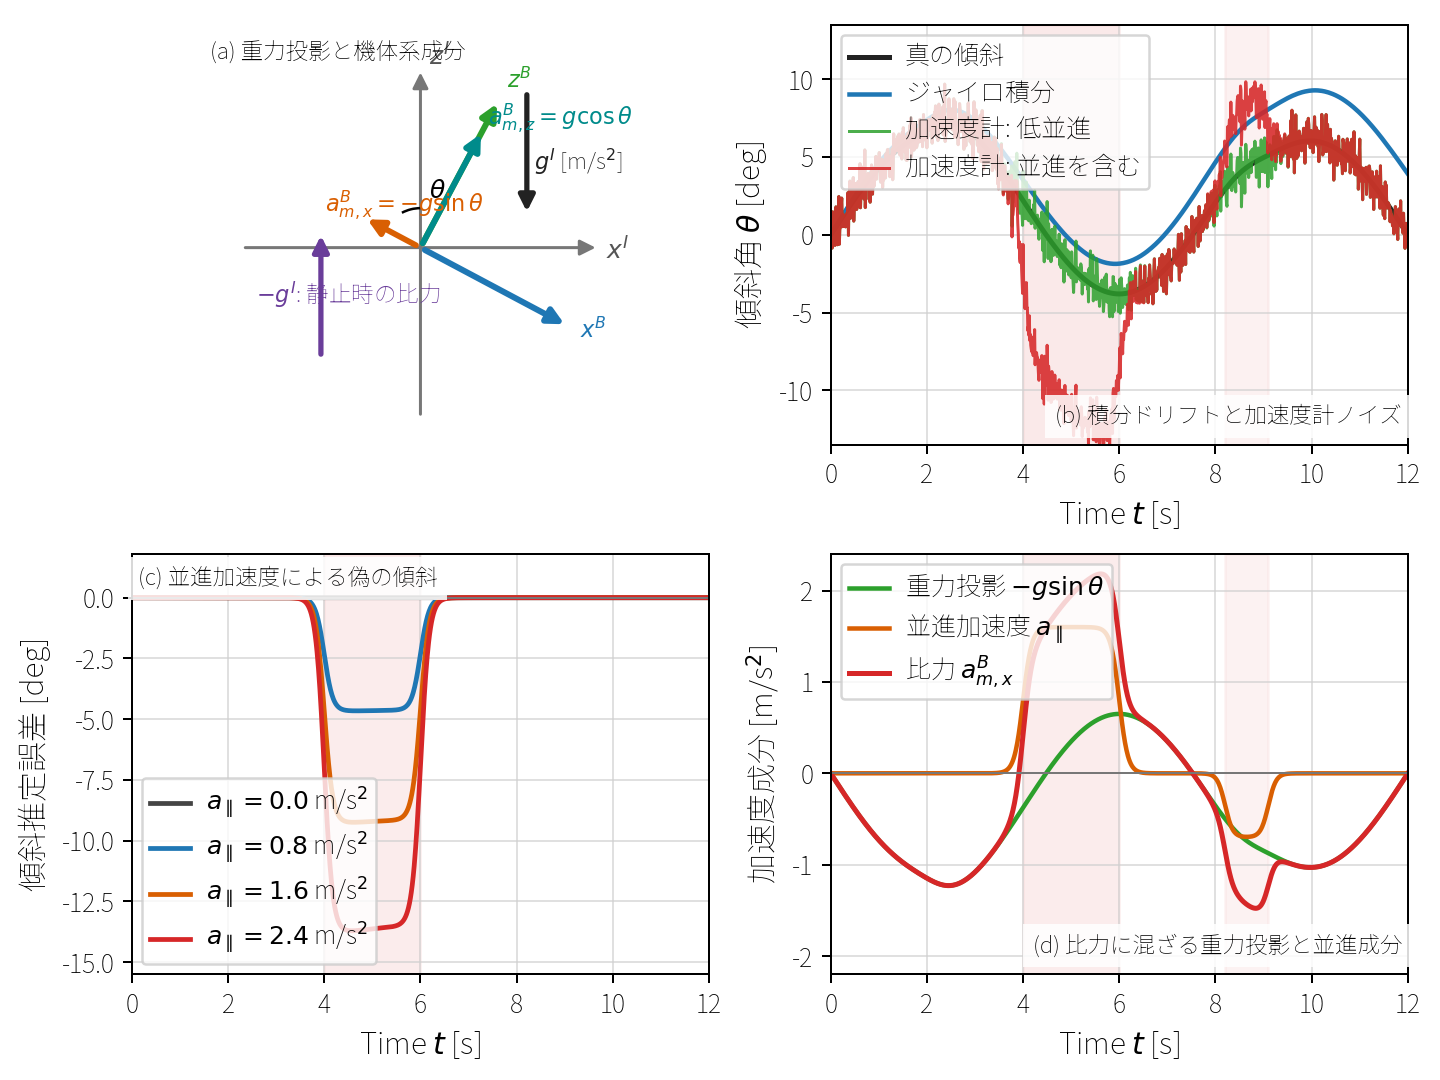
\includegraphics[width=0.95\linewidth,bb=0 0 1440 1080]{figures/flow6_accelerometer_tilt_examples.png}
\caption{加速度計による重力投影と傾斜推定の限界。左上は、静止時の比力が機体系の $x^B,z^B$ 軸へ投影され、$a_{m,x}^B=-g\sin\theta$、$a_{m,z}^B=g\cos\theta$ になる幾何である。右上は、真の傾斜、ジャイロ積分、低並進時の加速度計傾斜、並進加速度を含む加速度計傾斜を比較している。左下は $a_\parallel=0.0,0.8,1.6,2.4\,\mathrm{m/s^2}$ の変化による偽の傾斜誤差、右下は比力の $x$ 軸成分が重力投影と並進加速度の和として現れることを示す。}
\label{fig:flow6-accelerometer-tilt-examples}
\end{figure}

図\ref{fig:flow6-accelerometer-tilt-examples}の上段を比較すると、ジャイロ積分は短時間では滑らかに真の傾斜を追うが、一定の角速度バイアスによってゆっくりずれていく。加速度計から作った傾斜は積分を使わないのでバイアス性の角度ドリフトを持ちにくい一方、白色ノイズによって細かく揺れる。さらに、赤く示した並進加速度の時間帯では、式\eqref{eq:accelerometer-contaminated-tilt}の $a_\parallel/g$ に対応する誤差が乗り、実際には傾いていない向きの傾斜として推定される。下段のパラメータ変化では、$a_\parallel$ を大きくするほど偽の傾斜がほぼ比例して増え、$2.4\,\mathrm{m/s^2}$ では $14^\circ$ 程度のずれになる。

この結果から、ジャイロと加速度計は同じ角度を別々に測っているのではなく、互いに異なる弱点を持つ情報源であることが分かる。ジャイロ積分は高周波の姿勢変化を滑らかに保つが、低周波ではバイアスが角度ドリフトとして蓄積する。加速度計の重力投影は長時間の傾き基準を与えるが、ノイズと並進加速度に弱い。したがって次の段階では、低周波側では加速度計の重力基準を使い、高周波側ではジャイロ積分を使う相補フィルタを構成する。
